\section{Nombre: Jaguar}   \label{per:jaguar}
\subsection{Descripción:}
Felino de color amarillo con manchas negras. A pesar de ser un ser de propiedades mágicas, posee la apariencia de un jaguar común; sin embargo, posee un tamaño y una fuerza superior a éste.
\subsection{Status:}
\begin{itemize}
	\item Enemigo normal.
\end{itemize}
\subsection{Imagen}
Ver figura \ref{fig:jaguar}.
\begin{figure}
	\centering
	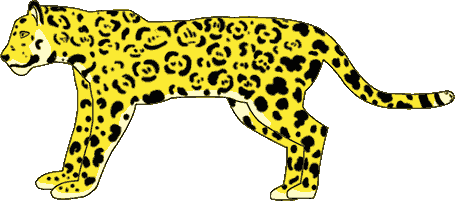
\includegraphics[height=0.2 \textheight]{Imagenes/jaguar}
	\caption{Concepto de diseño del Jaguar.}
	\label{fig:jaguar}
\end{figure}
\subsection{Encuentro:}
En el nivel 8 (ver apartado \ref{Nivel:Niv08}).
\subsection{Habilidades:}
\begin{itemize}
	\item Salto de altura (ver apartado \ref{hab.SalAl}).
\end{itemize}
\subsection{Patrón de ataque:}
El enemigo se desplazará del punto A al B utilizando la habilidad de embestida, permanecerá en el punto B por unos segundos en su estado de animación normal, después desplazará del punto B al A utilizando la habilidad de embestida, permanecerá en el punto A por unos segundos en su estado de animación normal. Este comportamiento se repetirá de manera cíclica.
\subsection{Bloques de animación:}
	\begin{itemize}
		\item Animación salto de altura.
		\item Animación normal.
	\end{itemize}